\documentclass[letterpaper,11pt]{article}

\usepackage{amsmath}
\usepackage{amssymb}
\usepackage{graphicx}
\usepackage{algorithm}
\usepackage{algorithmic}

\newcommand{\PM}{PYroMat}
\def\d{\mathrm{d}}

\title{The Thermodynamic Models in PYroMat}
\author{Christopher R. Martin}
\date{\today}

\begin{document}

\maketitle

\section{Introduction}

As of \PM\ version 2.1.0, there are three general model formulations used to evaluate the thermodynamic properties of gases and multi-phase (liquid-vapor) substances.  Each pure substance is referred to as a ``species.''  For ideal gases, calculating the properties of mixtures is almost trivial, but when inter-molecular forces rise to relevance, this task becomes difficult enough to require special treatment with a unique mixture model.

\section{Ideal Gases}

\subsection{Introduction}

In ideal gas models, inter-molecular forces are unimportant, so only the molecule's variable specific heat needs to be resolved in order to construct an entire thermodynamic model.  There are two classes in \PM\ for the two commonly used standards: the IG1 class manages the Shomate equation of state, and IG2 manages the so-called NASA polynomials equation of state.  In either case, constant-pressure specific heat, $c_p$, is constructed purely as a function of temperature.

When they are spread so sparsely that intermolecular forces between molecules are only relevant for the brief moments known as ``collisions,'' ideal gases are well described by the relation
\begin{align}
p = \rho R T.
\end{align}
$p$ is the pressure in Pa, $\rho$ is density in kg/m$^3$, R is the gas constant for the gas, and $T$ is the temperature in K.  When density is expressed in molar terms (usually called concentration) $R$ may be replaced by the universal gas constant, $R_u$.

In our treatment of gas properties, we will require the first law of thermodynamics, which states that energy must be conserved, and
\begin{align}
\delta q = \d e + p\d v.
\end{align}
Here, $q$ is heat in Joules, $e$ is the internal energy of the substance (energy stored in electrical, vibrational, chemical, nuclear, and translational energy of molecules) in Jounles per kilogram per Kelvin, $p$ is pressure in Pascals, and $v$ is specific volume (or $1/\rho$).  

Some will be irritated that $u$ is traditionally used for internal energy, but we have abandoned that tradition in an attempt (perhaps hopeless) to resolve some of the collisions in notation between fluid mechanics and thermodynamics.  We reserve $v$ for volume, $u$ for velocity, and $e$ for energy.  One possible objection might be that $e$ should be reserved for the natural number, which appears in many derivations.  Instead, we will always use the expression, $\exp()$, when we must.

The specific heat is the energy required to obtain a finite increase in temperature of finite amount of a substance.  When heat is applied in such a manner that the substance's volume is constant, $\d v = 0$, and
\begin{align}
\delta q |_v &= \d e\nonumber\\
 &= \left(\frac{\partial e}{\partial T}\right)_v \d T.
\end{align}
Thus, the constant-volume specific heat is, by definition, 
\begin{align}
c_v \equiv \left(\frac{\partial e}{\partial T}\right)_v.
\end{align}

In an ideal gas, $c_v$ is treated as \emph{only} a function of temperature, so we may drop the specification of constant-volume.  Much could be said about this assumption; it implicitly assumes that when a system of colliding molecules come to equilibrium, the fraction of internal energy expressed in translational kinetic energy does not depend on how tightly packed the molecules are.  This goes hand-in-hand with the assumption that intermolecular forces need not be modeled in detail.

When one considers addition of heat under constant pressure, a trick application of the chain rule for the term, $pv$, lets us transition the differential on volume into a differential on pressure.  The definition for enthalpy, $h=e+pv$, appears naturally.
\begin{align}
\delta q &= \d e + p \d v + v\d p - v \d p\nonumber\\
 &= \d(e + pv) - v\d p
\end{align}
To engineers practiced in the arts of fluid power system design will immediately recognize $pv$ as the term quantifying the mechanical energy carried by a flowing fluid.  Including it alongside $e$ merely means that we are accounting for mechanical energy communicated by the bulk material alongside the energy stored in the individual molecules of the substance.

Of course, when pressure is constant, $\d p=0$, and 
\begin{align}
\delta q |_p &= \d h\nonumber\\
 &= \left( \frac{\partial h}{\partial T}\right)_p \d T
\end{align}
Thus, constant-pressure specific heat is, by definition,
\begin{align}
c_p &\equiv \left( \frac{\partial h}{\partial T}\right)_p.\\
 &= \left(\frac{\partial e}{\partial T}\right)_p + \left(\frac{\partial (pv)}{\partial T}\right)_p.
\end{align}
We have already established that, for an ideal gas, internal energy is only a function of temperature, and $pv = RT$.  So,
\begin{align}
c_p(T) = c_v(T) + R,
\end{align}
and $c_p$ is also only a function of temperature.

Calorimetry provides means by which the specific heats of gases may be very precisely measured under different conditions.  So, provided with a sufficiently accurate function for specific heat, it is possible to calculate the other properties by its integral.

Enthalpy is readily calculated from $c_p$,
\begin{align}
h^\circ(T) &= \Delta h^\circ_f(T_{ref}) + \int_{T_{ref}}^T c_p(\tau) \d \tau.\label{eqn:ig:enthalpy}
\end{align}
The notation $h^\circ$ emphasizes that this is the enthalpy at standard pressure (usually 1bar for ideal gas data), but $h$ may be presumed to be insensitive to pressure so long as the ideal gas assumption holds.  

The integration constant, $\Delta h^\circ_f$, is called the enthalpy of formation.  It describes the enthalpy consumed when forming the species from other ``reference'' species.  Reference species (like O$_2$, N$_2$, H$_2$, C(s), He, Ar, Kr, and others) are arbitrarily defined to have zero enthalpy at 298.15K and 1bar, and calorimetry experiments including reactions with them allow the enthalpies of all other species to be constructed.  The enthalpy of formation is expressed in terms of the reference temperature, since the choice of reference temperature is arbitrary.  It is common to use $T_{ref} = 298.15$K.

There is a similar expression for standard entropy, which can be obtained from the definition of entropy and the first law.  For an ideal gas,
\begin{align}
\d s &= \frac{\delta q}{T} = \frac{\d h}{T} - \frac{v \d p}{T}\nonumber\\
 &= c_p \frac{\d T}{T} - R \frac{\d p}{p}.
\end{align}
The definition for enthalpy had no absolute zero reference, so we had to construct one from a convention.  However, the entropy for a substance \emph{can} be defined as zero when absolute temperature is zero.  Therefore, it is possible to define the entropy at a reference temperature and pressure.
\begin{align}
s^\circ(T_{ref},p_{ref}) &= \int_0^T \frac{c_p(\tau)}{\tau} \d \tau
\end{align}
From that state,
\begin{align}
s(T,p) &= s^\circ(T_{ref},p_{ref}) + \int_{T_{ref}}^T \frac{c_p(\tau)}{\tau} \d T - \int_{p_{ref}}^p \frac{R}{\pi} \d \pi\nonumber\\
&= s^\circ(T_{ref},p_{ref}) + \int_{T_{ref}}^T \frac{c_p(\tau)}{\tau} \d \tau - \ln\left(\frac{p}{p_{ref}}\right)\label{eqn:ig:entropy}
\end{align}

\PM\ calculates $s(T,p)$, but tables usually only list entropy as a function of temperature.  Why?  Since the pressure contribution to entropy can be calculated explicitly, the ``standard enthalpy,'' $s^\circ$, is normally what is tabulated,
\begin{align}
s^\circ(T) = s(T,p_{ref}) = s^\circ(T_{ref},p_{ref}) + \int_{T_{ref}}^T \frac{c_p}{T} \d T.
\end{align}

Note that we could propose conditions at pressures so large, $s(T,p)$ would evaluate to be zero or even negative.  Long before that occurs, the ideal gas assumption would be violated.  At such extreme densities, intermolecular forces would become relevant, and this expression would be beyond the scope of its usefulness.

Once $c_p(T)$ and $h(T)$ are well defined, it is also possible to evaluate internal energy,
\begin{align}
e(T) = h(T) - RT,
\end{align}
constant-volume specific heat,
\begin{align}
c_v(T) = c_p(T) - R,
\end{align}
specific heat ratio,
\begin{align}
\gamma(T) = \frac{c_p(T)}{c_p(T) - R},
\end{align}
speed of sound
\begin{align}
a(T) = \sqrt{\gamma(T) R T},
\end{align}
and others.

The central problem, then, is how to calculate $c_p(T)$.

As becomes clear in the next sections, polynomials are important to these formulations; so much so that we devote a separate section to their efficient evaluation.

\subsection{IG1: The Shomate Equation}

\PM's IG1 class is built on the Shomate equation for constant-pressure specific heat $c_p$.  This is the formulation used by the NIST/JANAF thermophysical property database.

The Shomate equation takes the form
\begin{align}
t &= \frac{T}{T_s}\\
c_p(t) &= c_0 + c_1 t + c_2 t^2 + c_3 t^3 + \frac{c_4}{t^2},
\end{align}
where the scaling temperature, $T_s$ is 1000K for all species.  Reducing the argument to the polynomial, $t$, to by on the order of 1 is an intelligent step to help reduce numerical errors, but it should be obvious that there is no attempt to base the formulation on fundamental physics.  This is a purely empirical formula.  Physics-based expressions for the specific heat of gases are available, but they become so numerically cumbersome, equations as simple as these are far preferable when available.

Because of its simplicity, the Shomate equations lacks the degrees of freedom to express specific heat over wide ranges, so data are usually given in piece-wise formulations.  For example, tungsten dioxide (WO$_2$), has a set of coefficients for $298\mathrm{K} \le T < 1100\mathrm{K}$ and $1100\mathrm{K} \le T \le 6000\mathrm{K}$.

The enthalpy can be explicitly calculated from (\ref{eqn:ig:enthalpy}),
\begin{align}
h(T) &= h_0 + \int c_p(T) \d T \nonumber\\
 &= h_0 + T_s \int c_p(t) \d t \nonumber\\
 &= T_s \left(c_0 t + \frac{c_1}{2} t^2 + \frac{c_2}{3} t^3 + \frac{c_3}{4} t^4 - \frac{c_4}{t} + c_5 \right).
\end{align}
It is important to emphasize that $h_0$ is not the same as the enthalpy of formation, $\Delta h^\circ_f$.  Instead, it is merely an integration constant, which can be alternately expressed as a new coefficient, $c_5$.

Because of the temperature term in the denominator, no multiple of $T_s$ appears in entropy when the integration is changed to $t$,
\begin{align}
s(T,p) &= s^\circ(T_{ref}) + \int_{T_{ref}}^T \frac{c_p(\tau)}{\tau}\d \tau - R \ln \left( \frac{p}{p_{ref}} \right)\nonumber\\
 &= s^\circ(T_{ref}) + \int_{T_{ref}}^T \frac{c_p(\tau)}{\tau}\d \tau - R \ln \left( \frac{p}{p_{ref}} \right)\nonumber\\
s(T,p) &= c_0 \ln t + c_1 t + \frac{c_2}{2} t^2 + \frac{c_3}{3} t^3 -\frac{c_4}{2t^2} + c_6 - R \ln\left(\frac{p}{p_{ref}}\right).
\end{align}
Just like in the enthalpy integral, a new coefficient, $c_6$, has been introduced to represent the integration constant.

Internal energy is readily calculated from the definition of enthalpy in (\ref{eqn:enthalpy}),
\begin{align}
e(T) &= h(T) - RT\nonumber\\
\end{align}
There is a similarly simple relationship to determine constant-volume specific heat and specific heat ratio,
\begin{align}
c_v(T) &= c_p(T) - R\\
\gamma(T) &= \frac{c_p(T)}{c_p(T)-R}
\end{align}

\subsection{IG2: The NASA polynomial}

Like the Shomate equation, the NASA polynomials are a piece-wise empirical formulation to the specific heat of an ideal gas.  Unlike the Shomate equation, there is no $1/t^2$ term, they make no attempt to scale temperature prior to evaluating the polynomial, and they are scaled with respect to the species' ideal gas constant.

\begin{align}
\frac{c_p(T)}{R} = R \left(c_0 + c_1 T + c_2 T^2 + c_3 T^3 + c_4 T^4\right)
\end{align}

There are nearly identical formulations for enthalpy,
\begin{align}
h(T) = R \left(c_0 T + \frac{c_1}{2} T^2 + \frac{c_2}{3} T^3 + \frac{c_3}{4} T^4 + \frac{c_4}{5}T^5 + c_5 \right),
\end{align}
and entropy
\begin{align}
s(T) = R \left(c_0 \ln(T) + c_1 T + \frac{c_2}{2} T^2 + \frac{c_3}{3} T^3 + \frac{c_4}{4} T^4 + c_6\right).
\end{align}
Here, just as in the Shomate equations, $c_5$ and $c_6$ are introduced as integration constants in enthalpy and entropy.

Internal energy is readily calculated from the definition of enthalpy in (\ref{eqn:enthalpy}),
\begin{align}
e(T) &= h(T) - RT\nonumber\\
\end{align}
There is a similarly simple relationship to determine constant-volume specific heat and specific heat ratio,
\begin{align}
c_v(T) &= c_p(T) - R\\
\gamma(T) &= \frac{c_p(T)}{c_p(T)-R}
\end{align}

\section{Multi-phase properties}

\section{Efficiently evaluating polynomials and their derivatives}

It must be clear from the previous sections that polynomials are an important tool for accurately modeling thermodynamic properties.  However, how they are best evaluated in code is more nuanced than it may seem.  

For example, if we were to evaluate $x^4$, we might use ``x**4'' in Python or we might use ``x*x*x*x''.  Which is better?  The answer depends on how much data we are analyzing.  Recall that \PM\ supports arrays.

Figure \ref{fig:benchmark} shows the results of a computation time study on the time to multiply Numpy arrays of different sizes.  The ``**'' and ``np.power'' operations were shown to be equivalent.  Certainly on faster or slower processors, the time scale might be faster or slower, but the shape of the curve should be roughly the same.

\begin{figure}
\centering
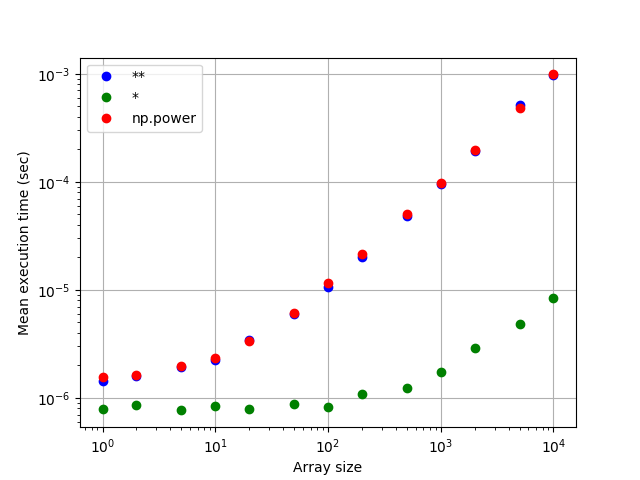
\includegraphics[width=.97\linewidth]{benchmark}
\caption{Computation time for array multiplication, and power operations.}\label{fig:benchmark}
\end{figure}

For small data sets (fewer than 10 or so elements), the overhead associated with Python being an interpreted language dominates the computational time, so adding array elements has little or no impact.  We could probably only perform two or three multiplications before the costs start to appear equal.  On the other hand, the computational costs are so small in these cases, it probably doesn't matter whether we use multiplication or exponents.

The real cost appears when data sets are larger.  By the time the arrays are over 1,000 elements, it is clear that multiplication and exponents diverge in their cost.  On a 10,000 element array, 100 multiplications can be performed for the cost of a single exponent and that trend only worsens with larger arrays.

The conclusion is that exponents should be used rarely (if ever) and repeated multiplications are dramatically more efficient.  This is somewhat less true on small data sets where there is significant computational overhead, but these operations are also so inexpensive to begin with, that there is little pressure on the optimization of the code.

The remaining question is how best to minimize the number of multiplications.

\subsection{Polynomials of one variable}

Polynomials of one variable may be expressed
\begin{align}
p(x) = c_0 + c_1 x + c_2 x^2 + c_3 x^3 + \ldots
\end{align}
We have made the case that it is preferable to express $x^3$ as $x\times x\times x$, but if that is the case, $x \times x$ would already have been available when calculating $x^2$, so we should absolutely avoid redundant operations.  An $N^\mathrm{th}$ order polynomial would imply $N(N-1)$ multiplications and $N$ additions.  On the other hand, if the polynomial were to be evaluated as
\begin{align}
p(x) = c_0 + x(c_1 + x(c_2 + x(c_3 + \ldots
\end{align}
there are only $N$ multiplications and $N$ additions.

While numerically expedient, it leads to a very awkward notation.  Instead, consider the polynomial constructed as a series.  For an $N^\mathrm{th}$ order polynomial,
\begin{subequations}
\begin{align}
\eta_N(x) &= c_N\\
\eta_k(x) &= c_k + x\eta_{k+1}(x) \hspace{1em} \forall\ k\ :\ 0 \le k < N\\
\eta_0(x) &= p(x).
\end{align}
\end{subequations}
This formulation invites an approach for calculating the polynomial numerically, but it also suggests a convenient method for efficiently calculating the derivative of the polynomial.
\begin{subequations}
\begin{align}
\eta'_N(x) &= 0\\
\eta'_k(x) &= \eta_{k+1}(x) + x\eta'_{k+1}(x)\\
\eta'_0(x) &= p'(x)
\end{align}
\end{subequations}
This operation requires $N$ additional multiplications and $N$ additional additions.

The same approach may be extended to a second derivative,
\begin{subequations}
\begin{align}
\eta''_N(x) &= 0\\
\eta''_k(x) &= 2\eta'_{k+1}(x) + x\eta''_{k+1}(x)\\
\eta''_0(x) &= p''(x),
\end{align}
\end{subequations}
\subsection{Polynomials of two variables}
and again, only $N$ additions and multiplications are added to the operation.

In the evaluation of empirical thermodynamic properties, there is often the problem of evaluating polynomial expansions on two variables.  These expansions are typically of the form
\begin{align}
p(x,y) = \sum_{i,j} c_{i,j} x^i y^j\label{eqn:general}
\end{align}
where $a$ and $b$ are real coefficients such that $i$ and $j$ are integer indices.

\subsection{Modifying polynomials for non-integer and negative powers}
Fractional and negative exponents are also possible within this framework if we were to accept input values $X$, and $Y$, and adjust them according to pre-exponentials $a$ and $b$,
\begin{align}
x &= X^a\\
y &= Y^b.
\end{align}
The new polynomial formed is
\begin{align}
p(X,Y) = \sum_{i,j} c_{i,j} X^{ai} Y^{bj}.
\end{align}
For example, were $a=0.25$, then the expansion on $X$ could proceed in fractions of 4 even though the evaluation algorithm we use is purely expressed in integer exponents.  It is relatively computationally inexpensive to apply these exponentials prior to the code's execution.  It would be far more costly to apply them to each term.

Similarly, negative exponentials can be achieved by using post-exponential terms
\begin{align}
P(X,Y) = X^\alpha Y^\beta p(X,Y).
\end{align}
When $\alpha$ or $\beta$ are non-zero, the effective exponents are all shifted positively or negatively by a single multiplication operation.

\subsection{Efficient evaluation of the polynomial}

The PYroMat polynomial evaluation algorithm is an expansion with purely integer exponents.
\begin{align}
p(x,y) = \sum_{i,j} c_{i,j} x^i y^j
\end{align}
However, evaluating each term individually requires two expensive calls to a \verb|pow| function and two floating point multiplications.

The widely accepted method for evaluating a polynomial of one variable is to construct a recursive expansion
\begin{align}
q(y) = c_0 + y ( c_1 + y ( c_2 + y ( \ldots
\end{align}
If there are $n$ coefficients, then this amounts to only $m$ multiplications with no \verb|pow| calls.  In order to extend this algorithm to two variables, more elegant notation will be helpful.  If we name the intermediate value calculated in the process of these recursions $q$, then a polynomial with $n$ terms implies the series
\begin{align}
q_n &= c_n\\
q_j(y) &= c_j + y\,q_{j+1}(y)\\
q_0(y) &= q(y).
\end{align}
This is a series beginning with $q_n$, and proceeding backwards through the values of $j$ to $q_0$, which is the final value for $q(y)$.  In practice, there is no need to keep the old values of $q$, so a single register may be used to hold the latest value.

How can this be extended to a polynomial of two variables?  We may consider the polynomials to be nested; the evaluation of a polynomial on $Y$ determines the individual coefficients for a polynomial on $X$.
\begin{align}
p(x,y) &= \sum_i q_i(y) x^i\\
q_i(y) &= \sum_j c_{i,j} y^j
\end{align}

We only need a minor modification to the intermediate values for the $x$ polynomial since there will be a separate expansion for each value of $i$.  If there are $n$ $j$ terms,
\begin{subequations}
\begin{align}
q_{i,n}(y) &= c_{n,j}\\
q_{i,j}(y) &= c_{i,j} + y\,q_{i+1,j}(y)\\
q_{i,0}(y) &= q_i(y).
\end{align}
\end{subequations}

If there are $m$ $x$ terms,
\begin{subequations}
\begin{align}
p_m(x) &= q_m(x)\\
p_i(x,y) &= q_i(x) + y\,p_{i+1}(x,y)\\
p_0(x,y) &= p(x,y).
\end{align}
\end{subequations}

\subsection{Efficient evaluation of derivatives}
The partial derivatives of the polynomial can be efficiently evaluated along with the polynomial itself. To relax the already cumbersome notation, the functional dependencies $(y)$ and $(x,y)$ will be dropped.  For the purpose of thermodynamic property evaluation, the first two derivatives will suffice.

Let us begin with the simpler task of calculating the derivatives of $q_j$.
\begin{subequations}
\begin{align}
q_{i,n|y} &= 0\\
q_{i,j|y} &= q_{i+1,j} + y\,q_{i+1,j|y}\\
q_{i,0|y} &= q_{i|y}
\end{align}
\end{subequations}

\begin{subequations}
\begin{align}
q_{i,n|yy} &= 0\\
q_{i,j|yy} &= 2 q_{i,j+1|y} + y\,q_{i,j+1|yy}\\
q_{i,0|yy} &= q_{i|yy}
\end{align}
\end{subequations}

The derivatives on $p$ are constructed somewhat differently because they can be in both $x$ and $y$.  Beginning with $y$,
\begin{subequations}
\begin{align}
p_{n|y} &= 0\\
p_{j|y} &= q_{i|y} + x\,p_{j+1|y}\\
p_{0|y} &= p_y
\end{align}
\end{subequations}

\begin{subequations}
\begin{align}
p_{m|yy} &= 0\\
p_{i|yy} &= q_{i|yy} + x\,q_{i+1|yy}\\
p_{0|yy} &= p_{yy}
\end{align}
\end{subequations}

The derivatives on $x$ appear
\begin{subequations}
\begin{align}
p_{m|x} &= 0\\
p_{i|x} &= p_{i+1} + x\,p_{i+1|x}\\
p_{0|x} &= p_x
\end{align}
\end{subequations}

\begin{subequations}
\begin{align}
p_{n|xx} &= 0\\
p_{i|xx} &= 2 p_{i+1|x} + x\,p_{i+1|xx}\\
p_{0|xx} &= p_{xx}
\end{align}
\end{subequations}

Finally, the cross-term (both $x$ and $y$) appears
\begin{subequations}
\begin{align}
p_{n|xy} &= 0\\
p_{i|xy} &= p_{i+1|y} + y\,p_{i+1|xy}\\
p_{0|xy} &= p_{xy}
\end{align}
\end{subequations}

\subsection{Implementation of the algorithm}
In practice, this cumbersome notation can be drastically simplified in code because it is not necessary to distinguish between $p$ and $q$ in their various incarnations; provided care is taken not to overwrite a value before it is needed.

In most practical polynomials of two variables of given order, very few of the possible coefficients may be non-zero, so storing and looping over all $m\times n$ coefficients may not be sensible.  Instead, it is common to take an approach closer to spare matrix storage.

If we have one-dimensional arrays of polynomial coefficients, $c_k$, and exponents, $a_k$ and $b_k$, the polynomial will be constructed as
\begin{align}
p(X,Y) = \sum_k=0^{N-1} c_k X^{a_k} Y^{b_k}.
\end{align}
In this way, the polynomial
\begin{align}
p(X,Y) = -0.1 X^2 + XY + 0.5 Y^2 - Y - 0.2
\end{align}
may be represented by
\begin{align}
a &= \left[ 2,\ 1,\ 0,\ 0,\ 0\right]\\
b &= \left[ 0,\ 1,\ 2,\ 1,\ 0\right]\\
c &= \left[ -0.1,\ 1,\ 0.5,\ -1,\ 0.2\right]
\end{align}

For the algorithm to function efficiently, it is reasonable to impose some prior sorting of the exponent values.  Since the series above requires that we interact with higher-order terms first, let us assert that the polynomial should be expressed in order of descending exponents on $X$ and then $Y$.

In Algorithm \ref{alg:poly2}, we employ an outer loop on the values of $i$ and an inner loop on the values of $j$.  If coefficients are absent from the arrays (if the $i,j$ pair is not found), then the coefficient is presumed to be zero.  Starting with the maximum value for each exponent, the indices are reduced incrementally until the $i,j$ combination corresponding to the next row ($k$) is found.

This is extremely practical for polynomials where most of the possible combinations are not represented, and does not cost much for cases where they are.

\begin{algorithm}
\caption{Efficient evaluation of a polynomial of two variables}\label{alg:poly2}
\begin{algorithmic}[1]
\REQUIRE $a,b,c \in \mathbb{R}^N$
\REQUIRE The coefficient order is sorted in descending order of $a$ and then $b$ so that\\
$a_k \ge a_{k+1}\ \forall\ k \in [0,N-1)$\\
$b_k > b_{k+1}\ \forall\ k : a_k = a_{k+1}$
\ENSURE $p$, $p_x$, $p_y$, $p_{xx}$, $p_{xy}$, $p_{yy}$ are equal to the polynomial and its derivatives.

\STATE $p, p_x, p_y, p_{xx}, p_{xy}, p_{yy} \leftarrow 0$
\STATE $i_{max} \leftarrow a[0]$
\STATE $k \leftarrow 0$
\FOR{$i=i_{max}$ to $0$}
    \IF{$k < N$ \AND $a_k$ equals $i$}
        \STATE $j_{max} \leftarrow b_k$
        \STATE $q,q_y,q_{yy} \leftarrow 0$
        \FOR{$j=j_{max}$ to $0$}
            \STATE $q_{yy} \leftarrow 2 q_y + y q_{yy}$
            \STATE $q_y \leftarrow q + y q_y$
            \IF{$k<N$ \AND $a_k$ is $i$ \AND $b_k$ is $j$}
                \STATE $q \leftarrow c_k + y q$
                \STATE $k \leftarrow k+1$
            \ELSE
                \STATE $q \leftarrow y q$
            \ENDIF
        \ENDFOR
        \STATE $p_{yy} \leftarrow q_{yy} + x p_{yy}$
        \STATE $p_{xx} \leftarrow 2 p_x + x p_{xx}$
        \STATE $p_{xy} \leftarrow p_y + x p_{xy}$
        \STATE $p_x \leftarrow p + x p_x$
        \STATE $p_y \leftarrow q_y + x p_y$
        \STATE $p \leftarrow q + x p$
    \ELSE
        \STATE $p_{yy} \leftarrow x p_{yy}$
        \STATE $p_{xx} \leftarrow 2 p_x + x p_{xx}$
        \STATE $p_{xy} \leftarrow p_y + x p_{xy}$
        \STATE $p_x \leftarrow p + x p_x$
        \STATE $p_y \leftarrow x p_y$
        \STATE $p \leftarrow x p$
    \ENDIF
\ENDFOR
\end{algorithmic}
\end{algorithm}
\end{document}
